\documentclass[8.5pt,twoside,twocolumn]{article}
%% CHECK: Remove all ``CHECK'' comments by solving their problems
\usepackage[utf8]{inputenc}
\usepackage{MyChem}
\usepackage{MyStandard}
\usepackage{courier}
\usepackage{booktabs}
%%\usepackage{tabto}
%% \usepackage{tabu}
\usepackage{longtable}
\usepackage{enumerate}

\usepackage[justification=justified,singlelinecheck=false,
 aboveskip=0em,belowskip=0em]{caption}


\usepackage{tikz}
\usepackage{pgfplots}
\usepackage{rotating}
\usepackage{verbatim}
\usetikzlibrary{patterns,calc,decorations.pathmorphing,angles,quotes,external}
\tikzexternalize[shell escape=-enable-write18]

\makeatletter
\newcommand{\subalign}[1]{%
  \vcenter{%
    \Let@ \restore@math@cr \default@tag
    \baselineskip\fontdimen10 \scriptfont\tw@
    \advance\baselineskip\fontdimen12 \scriptfont\tw@
    \lineskip\thr@@\fontdimen8 \scriptfont\thr@@
    \lineskiplimit\lineskip
    \ialign{\hfil$\m@th\scriptstyle##$&$\m@th\scriptstyle{}##$\crcr
      #1\crcr
    }%
  }
}
\makeatother

\newcommand\snakedeko{{snake, segment length=1.5mm, amplitude=.5mm}}

\newcommand\eint{\enmat{E^{\te{int}}}}
\newcommand\eads{\enmat{E^{\te{ads}}}}
\newcommand\ezp{\enmat{E^{\te{ZPE}}}}
\newcommand\dft{\enmat{_{\te{DFT}}}}

\renewcommand\Hil{\enmat{\mathcal H_a}}

\renewcommand\H{\enmat{\bo H}}

\newcommand\di{\te{d}}
\newcommand\dr{\di\r}
\newcommand\drr{\di\r\ }
\renewcommand\ij{_{ij}}
\newcommand\rms{\te{RMS}}
\newcommand\apd{\te{APD}}
\renewcommand\K{{\enmat{~\te{K}}}}
\renewcommand\r{\bo r}
\newcommand\ri{\enmat{\r_i}}
\newcommand\rip{\enmat{\r_{i'}}}
\newcommand\indr{\enmat{\int\di \r}}

\newcommand\kmo{\enmat{\te {kJ/mol}}}
\newcommand\id{\hskip.2cm}
\newcommand\pab{\enmat{\phi_{AB}}}



\newtheoremstyle{standard}{10 pt}{10 pt}{\hangindent=0.25in\itshape}{}{\normalfont\bfseries}{}{\newline}{}
\theoremstyle{standard}
\newtheorem{theo}{Theorem}
\newtheorem{lem}[theo]{Lemma}
\newtheorem{res}[theo]{Result}
\newtheorem{defi}[theo]{Definition}
\newtheorem{exm}[theo]{Example}
\newtheorem{cor}[theo]{Corollary}

%% FROM http://tex.stackexchange.com/questions/159139/what-is-required-to-use-background-layer-as-specified-in-tikz-manual
\pgfdeclarelayer{background}
\pgfdeclarelayer{foreground}
\pgfsetlayers{background,main,foreground}  

%% GRAPH COMMANDS
\newcommand\fp[2]{\draw {#1} node[circle,minimum size=0.2cm,draw,fill=black]
({#2}) {};} %field point
 \newcommand\lp[2]{\draw {#1} node[circle,minimum size=0.2cm,draw,fill=white]
({#2}) {};} % labelled point
\newcommand\flp[2]{\draw {#1} node[circle,minimum
size=0.2cm,draw,dashed,fill=white] ({#2}) {};} %free labelled point
\newcommand\connect[1]{
\begin{pgfonlayer}{background}
 \foreach \x/\y in {#1} {\draw (\x.center) -- (\y.center);}
\end{pgfonlayer}
}

\newcommand{\itemEq}[1]{%
        \begingroup%
        \setlength{\abovedisplayskip}{0pt}%
        \setlength{\belowdisplayskip}{0pt}%
        \parbox[c]{\linewidth}{\begin{flalign}#1&&\end{flalign}}%
        \endgroup}


\parindent0pt

\linespread{1.5}
\title{Surface Adsorption on Interstellar Ice $I_h$}
\linespread{1}
% \subtitle{Universit�t Stuttgart, Prop�deutikum zur Bachelorarbeit}
\author{T. Bissinger}

\begin{document}


\begin{titlepage}

\begin{center}

% Oberer Teil der Titelseite:

 

% Title

\newcommand{\HRule}{\rule{\linewidth}{0.5mm}}

\HRule \\[0.4cm]

{ \huge \bfseries Surface Adsorption on Interstellar Ice $I_h$}


\HRule \\[2cm]

{\LARGE Thomas Bissinger}\\[4cm]

\vfill 
%% CHECK: Stuttgart Figure
[width=7cm]{./Figures/unistuttgart.jpg}\\[2cm]   

{\Large Master Thesis supervised by \\[.7cm]
Prof. Dr. rer. nat. J. Kästner \\[.4cm]
M. Sc. Jan Meisner}\\[.4cm]


{ \Large  Institute for Theoretical Chemistry, Universität Stuttgart, December 2015}


% Author and supervisor

% Unterer Teil der Seite

\end{center}


\end{titlepage}
\newpage
\newpage
\clearpage



% \tableofcontents
% \newpage
\twocolumn[
	\maketitle
  \begin{@twocolumnfalse}
    \maketitle
    \begin{abstract}
      This abstract explains what happens. Benchmark, adsorption, maybe something about the interstellar playground.
\\
\\
    \end{abstract}
  \end{@twocolumnfalse}
]
\section{Introduction}
\label{Sec:Intro}
Interstellar chemistry is the key ingredient to understanding the molecular abundancies in our universe. While
the formation of atoms takes place in stars \cite{AtomsInStars}, their further reaction and therefore the composition
of molecular compunds in space largely happens in interstellar clouds. With modern telescopes it is possible to
measure the molecular abundancies in the interstellar medium (ISM) to a high degree of accuracy. It became
evident that the reaction rates governing the formation of molecules can not properly be explained by gas phase
chemistry alone. A prominent theory to mend this discrepancy is to consider the contribution of surface reaction
on interstellar dust grains. The dust has been measured \cite{DustMeasure}, so the question is not so much if the
reaction happens but rather to quantify its effect.

At temperatures as low as in cold interstellar clouds (between 10 and 100 $K$), the grains are covered in ices,
most prominently $\hto $ and $\co$. In the case of water, one faces \ep{amorphous solid water} (ASW), but
at very low temperatures one may find a state close to the crystalline $I_h$ state of frozen water.

Various works have already considered surface reactions.

(Here we will cite some experimentalists).

The research described above typically chose a model to describe the processes taking place in the experiment and
adjusted simulation data -- including parameters like the diffusion coefficient -- to fit the experimental data.
That would mean: if surface reaction processes are the key to filling the gap between observed and predicted
reaction rates, the input parameters might be good approximations to the actual coefficients. This is a legit
approach since one can not easily think of other processes than surface and gas phase reactions to lead to
molecular formation.

%% CHECK: Andere Parameter als Diffusionskoeffizient?
However, there is not yet a proper \ep{ab initio} theoretical calculation of surface diffusion. This means that
evaluating the parameters found in simulation is a very difficult task -- there is neither a recommended value nor 
are there any error bars to such a value. This work tries to make a first step toward the accurate simulation of surface
adsorption, diffusion and reaction of small molecules on interstellar ices. Its aim is to establish a model
of crystalline $I_h$ water in which simulations can be carried out. The main mathematical tool for describing the 
chemistry of this surface is a subdomain treated by \ep{density functional theory} (DFT) within a bigger domain
where the interaction is modelled by \ep{molecular mechanics} (MM). The two domains are coupled by a QM/MM
coupling scheme.

We will describe the theory underlying the model in the next section. Section \ref{Sec:Bench} then describes the
benchmarking we performed on smaller test systems to determine the best functionals and basis sets to use for 
the actual system. After that, we give our results for adsorption energies in Section \ref{Sec:Ads} and finally 
there will be concluding remarks and an outlook on possible further application for our findings in Section 
\ref{Sec:Con}.

\section{Theoretical Background}
\label{Sec:Theo}
This section focuses on the theoretical framework of the ice surface model. We introduce the main chemical
nomenclature in Section \ref{Sec:Theo:Interaction} and then proceed to the mathematical ideas behind
DFT in Section \ref{Sec:Theo:QMMet}. After that, Section \ref{Sec:Theo:MM} will explain how we describe
the MM interaction of the system and Section \ref{Sec:Theo:QMMM} explains how QM and MM are coupled
by the QM/MM procedure. Finally, Section \ref{Sec:Theo:Minima} describes how to find energy minima
of the potential energy surface.

\newcommand\X{\enmat{\te X}}
\newcommand\Y{\enmat{\te Y}}
\newcommand\XY{{\enmat{\X - \Y}}}
\renewcommand\S{\enmat{\te S}}
\newcommand\sX{\enmat{\te {s-X}}}
\newcommand\A{\enmat{\te A}}
\subsection{Different Types of Energy}
\label{Sec:Theo:Interaction}
We will consider the \ep{interaction energy} between two molecular species X and Y. We call
the system of both molecules $\XY$. We also consider the \ep{adsorption energy} of a molecule X on
the ice surface S. We call this system $\sX$. If not declared elsewise, all appearing energies are
electronic ground state energies. We wil describe the interaction energy first.

Consider a system of two molecules X and Y. We can calculate the energy of the isolated molecule X to
be $E_{\te X}$ and the energy of the isolated molecule Y to be $E_{\te Y}$. We can also calculate the 
energy of the full system $\XY$, which will in general depend on the distance and the orientation
of the two molecules, to be $E_{\XY}$. Then, the interaction energy between the two molecules
is the energy given by
\begin{equation}
 \eint_{\XY} := E_{\XY} - E_\X - E_\Y.
 \label{Theo:InteractionEnergy}
\end{equation}
We did not include spatial dependency of $E_{\XY}$ into the above definition. A map
\mbox{$(R_\XY, \Om_\X, \Om_\Y) \mapsto \eint_\XY$} with the center of mass separation
$R_\XY$ and the molecular orientation $\Om_\X$ and $\Om_\Y$ is called the \ep{potential energy surface} (PES)
of the intermolecular interaction. It may also contain internal deformations of the molecule.

However, one does often speak of the interaction energy of two molecules without further specification
of a point on the PES. This is usually a reference to the minimum geometry
of $\XY$, that is the global minimum of $E_{\XY}$ and therefore $\eint_\XY$. If the interaction between $\X$ and $\Y$
were purely repulsive, that is $\eint_{\XY} > 0$ for all geometries, the global minimum would
not be well-defined since it requires inifinite separation of $\X$ and $\Y$ in an arbitrary direction.
However, the algorithms we use will converge to a local minimum around the initial geometry we
specify, by which we will then classify the strength of the repulsion. Even for attractive potentials,
that is potentials where $\eint_\XY < 0$ for some geometries, we are not able to determine whether 
the potential energy minimum we find is the global minimum or within what error its energy is
to the global minimum.

The adsorption energy is mostly similar. There, we have the energy of the isolated species
$E_\X$ and the energy minimum of the surface $E_{\S}$. If we denote the system of the surface 
with the adsorbed molecule $X$ by $\sX$ and its energy minimum by $E_\sX$, we define
the adsorption energy to be
\begin{equation}
 \eads_{\sX}:= E_{\sX} - E_\X - E_\S.
 \label{Theo:AdsorptionEnergy}
\end{equation}
Again, we did not include the dependency of $E_\sX$ and $E_\S$ on the respective geometries. We
even specified that we will consider the individual geometry of minimum energy here. This is quite sensible
because the surface geometry of the system $\sX$ \mbox{(surface + molecule)} may be different from the
system $\S$ of the surface alone when comparing energy minima. For a fixed value of $E_\S$, 
we could again consider a PES of the type \mbox{$(\bo r_i)_i \mapsto \eads_\sX$}, where the
vector $\r_i$ is the coordinate of the $i$-th atom in $\sX$, $1 \le i \le N$ for some $N$. The different energy minima of 
this map to $\eads_\sX$ are called \ep{binding geometries}, and the position of the
center of mass of the molecule $\X$ in a binding geometry is called a \ep{binding site}.
Exploring binding sites and the strength of the binding $\eads_\sX$ can be useful
to simulation.

The superscripts on $\eint$ and $\eads$ may be ignored if it is sufficiently clear which energy 
is meant.

We also want to introduce a third type of energy, the \ep{zero-point (vibrational) energy}.
We describe it for some general system $\A$ that may contain any arrangement of atoms.
For all calculations we do, we will work with fixed values for the atomic coordinates
$\r_i$, $1 \le i \le N$ for some $N \in \N$. That description can only be accurate if
the atoms were classical particles. However, if we want to allow for them to be
quantum objects, we need to include uncertainty into their position. This is usually
done by including the zero-point vibrational energy of the atoms. It is computed from the
\ep{Hessian} matrix $\H$ of the system,
\begin{equation}
 \H(\r_1,\ldots,\r_N) := \rb{\deri {^2 E} {\r_i \del \r_j} (\r_1,...,\r_N) }_{1\le i,j \le N}
 \label{Theo:Hessian}
\end{equation}
by
%% CHECK: Is this correct?
\begin{equation}
 \ezp=E + \frac 1 2 \te {tr} \ed{\H} = E + \Dl \ezp,
 \label{Theo:EZP}
\end{equation}
where $\te {tr} \ed{\H}$ is the \ep{trace} of the matrix $\H$, that is the sum of the eigenvalues
of $\H$. In the harmonic approximation, which should be accurate for the vibrational ground 
state, the eigenvalues of $\H$ are 
%% CHECK: proportional or identical?
proportional
to the eigenfrequencies of the system. We call the term $\Dl \ezp$ the \ep{zero-point (vibratinal energy)
correction}.

We will always use the superscript in $\ezp$ if we want to denote energies that are corrected 
with $\Dl \ezp$ in \eqref{Theo:EZP}.

\subsection{Methods of Quantum Chemistry}
\label{Sec:Theo:QMMet}

We already saw a few different energy expressions so far. The accurate calculation of these 
is naturally vital to anything we want to do in this work. We now want to focus on the methods
of quantum chemistry which will be used to describe the quantum mechanical part of our system.

\subsubsection{Basics of Density Functional Theory}
For a system with a time-independent potential $V$, one usually looks for solution of the 
\ep{time-independent Schrödinger equation}
\begin{equation}
 \Ha \keP{} = E \keP{}.
 \label{Theo:Schroedinger}
\end{equation}
This equation holds for all non-relativistic quantum mechanical particles. Within the \ep{Born-Oppenheimer}
approximation, one can separate the dynamics of the atomic cores from the dynamics of the electrons. We will treat
the cores in a more or less classical way, therefore we will for now focus on solving the Schrödinger 
equation for $N < \infty$ electrons, that is the Hamiltonian of our system is
\begin{equation}
 \Ha = -\sum_{i=1}^N \frac{\hbar^2}{2m_e} \nabla_i^2 + \frac {e^2} {4 \pi \e_0} \sum_{1\le i < j \le N} \frac 1 {\abs{\r_i - \r_j}} + V(\r^N).
 \label{Theo:Hamiltonian}
\end{equation}
$\r_i$ is the space coordinate of electron $i$ and $\nabla_i^2$ is the \ep{Laplace operator} applied to the three coordinates contained in $\r_i$. 
The electrons move in an external potential $V$ given by the core geometry and movement, where $\r^N$ is the vector containing
all electron coordinates. We will have for $K < \infty$ atomic cores 
\begin{equation}
\begin{aligned}
V(\r^N)=&-\sum_{A=1}^K \frac{\hbar^2}{2m_A} \nabla_A^2 + \frac {e^2} {4 \pi \e_0} \sum_{A=1}^K \sum_{B=1}^K \frac {Z_A Z_B} {\abs{\bo R_A - \bo R_B}} \\
   &- \frac {e^2} {4 \pi \e_0} \sum_{A=1}^K \sum_{i=1}^N \frac {Z_A} {\abs{\bo R_A - \r_i}}. 
\end{aligned}
\label{Theo:CorePotential}
\end{equation}
Here, $Z_A$ is the atomic number of atom $A$ and $\bo R_A$ is the coordinate of it with corresponding $\nabla_A^2$. We
can separate $V$ into a core-core (cc) and an core-electron (ce) potential
\newcommand\vce{V_{\te{ce}}}
\newcommand\vcc{V_{\te{cc}}}
\begin{equation}
 V(\r^N)=\vcc+\vce(\r^N)
\label{Theo:SeparatePotential}
\end{equation}
with
\begin{equation}
 \vce(\r^N)=\sum_{i=1}^N \tilde V(\r_i) = - \frac {e^2} {4 \pi \e_0} \sum_{A=1}^K \sum_{i=1}^N \frac {Z_A} {\abs{\bo R_A - \r_i}}.
 \label{Theo:CoreElectronPotential}
\end{equation}



There will be more than one solution to \eqref{Theo:Schroedinger}, so one can construct the set of all solutions $\st{\keP{_i} | i \in \N_0}$
with corresponding energy eigenvalues $E_i$. $\st{\keP{_i}}$ always is the complete basis of
some $\mathbb C$-vector space $\Hil$, where the subscript $a$ denotes antisymmetry according 
to the \ep{Pauli principle}
\begin{equation}
\begin{aligned}
 &\bkt{\x_1,\ldots,\x_l,\ldots,\x_k,\ldots,\x_N | \Psi_i } \\
 &=\ph - \Psi_i(\x_1,\ldots,\x_l,\ldots,\x_k,\ldots,\x_N) \\
 &= - \Psi_i(\x_1,\ldots,\x_k,\ldots,\x_l,\ldots,\x_N),
\end{aligned}
\label{Theo:Pauli}
\end{equation}
where we used $\x_i=(\r_i,s_i)$ for orbital coordinates $\r_i$ and the spin coordinate $s_i$.

 If $\Hil \suseq \mathcal {L}^2$, which is usually the case,
the set of solutions can be chosen orthonormal $\bkt{\Psi_i | \Psi_j} = \dl_{ij}$.
The set of solutions is usually not finite and the set of eigenvalues (energies) $E_i$ of $\Ha$
is not necessarily bounded from above. But there is always a minimum energy, denoted by $E_0$, 
which we call the \ep{(electronic) ground state energy}. The corresponding eigenvector 
$\keP{_0}$ is the \ep{(electronic) ground state}. They can both be obtained by the
variational ansatz
\begin{equation}
\begin{aligned}
 E{_0}&= \min_{\keP{}} \st{ \brP{} \Ha \keP{}}, \\
 \keP{_0}&= \argmin_{\keP{}} \st{ \brP{} \Ha \keP{}}.
\end{aligned}
\label{Theo:Variation}
\end{equation}
Note that while $E_0$ is unique, there may be multiple possibilities for $\keP{_0}$, although
we will not consider that case.

Now, equation \eqref{Theo:Schroedinger} has a variety of equivalent counterparts. One of them
is the key to the approach of DFT. When multiplying \eqref{Theo:Schroedinger} by the bra $\brP{}$,
one can interpret the resulting energy as a (non-linear) functional of the wavefunction by
\begin{equation}
 E : \Hil \rar \R, \qquad E\ed{\keP{}}=\brP{} \Ha \keP{},
 \label{Theo:WaveFunctional}
\end{equation}
which would mean that the ground state energy can be found by minimizing the functional
$E\ed{\keP{}}$ according to \eqref{Theo:Variation}. But so far, the minimization
of said functional only differs in semantics from the task of minimizing the energy expectation value.

A truly new task arises from considering the \ep{electron density} $\rho$ instead of the wave function
$\Psi$. The two approaches are related, since the ground state electron density is given by
\begin{equation}
 \rho(\x_1,...,\x_N)=\abs{\Psi_0(\x_1,...,\x_N)}^2,
 \label{Theo:NElectronDensity}
\end{equation}
This $N$-electron density describes the probability of finding the system in a state within 
a small volume of $\di \x_1 \cdots \di \x_N$ around $(\x_1,\ldots,\x_N)$. 
The $N$-electron density can be reduced to the one-electron density by
\begin{equation}
 \rho(\r_1,s_1)=\int\di\x_2 \cdots \int\di \x_N \abs{\Psi_0(\x_1,...,\x_N)}^2,
 %\rho(\r_1)=\int\di s_1\int\di\x_2 \cdots \int\di \x_N \abs{\Psi_0(\x_1,...,\x_N)}^2,
 \label{Theo:1ElectronDensity}
\end{equation}
where the integrals run over %the spin of the first particle and
the full spin-orbit space for all particles but the first.

For a system of $N$ electrons, Hohenberg and Kohn \cite{HohenbergKohn} were able to show that the ground state
one-electron density uniquely determines the Hamiltonian except for the addition of a constant,
and that conversely there is a functional of the density that has its minimal value at the one-electron
ground state density, and for which the minimum value is the ground state energy. Therefore, the task
of solving the Schrödinger equation \eqref{Theo:Schroedinger} is reduced to the task of finding
the minimum of this density functional.

The problem here is that not much is known about the nature of this density functional. The
popular ansatz by Kohn and Sham \cite{KohnSham} is called Kohn-Sham (KS) DFT, and the energy
expression is given by
% CHECK: Role of \vcc
\newcommand\er{\ed{\rho}}
\newcommand\exc{E_{\te{xc}}}
\begin{equation}
\begin{aligned}
 E\ed{\rho}=&\vcc+\indr\ \tilde V(\r) \rho(\r) + \frac {e^2}{2}\indr\indr' \frac {\rho(\r)\rho(\r')}{\abs{\r-\r'}}\\
 &+T_s 	\ed{\rho}+\exc\ed{\rho}
\end{aligned}
\label{Theo:EnergyDensityFunctional}
\end{equation}
The two problematic terms that remain are the \ep{kinetic energy functional} $T_s\er$ and the
\ep{exchange correlation functional} $\exc\er$. The former is treated in the Kohn-Sham approach
by  introducing \ep{Kohn-Sham orbitals} $\phi_i$ that solve the equations
\newcommand\veff{V_{\te{eff}}}
\newcommand\hm{\frac{\hbar^2}{2m}}
\begin{equation}
\rb{-\frac{\hbar^2}{2m} \nabla^2 + \veff(\r)} \phi_i(\r) = \eps_i \phi_i(\r)
\label{Theo:SCFDFT}
\end{equation}
with the \ep{effective potential}
\begin{equation}
\veff(\r)=\vcc+V(\r) + \frac {e^2}2 \indr' \frac{\rho(\r')}{\abs{\r-\r'}}+\delti{\exc\er}{\rho(\r)}.
\label{Theo:Veff}
\end{equation}
The latter term is often expressed by the \ep{exchange correlation potential}
\newcommand\vxc{V_{xc}}
\begin{equation}
\vxc=\delti{\exc\er}{\rho(\r)}.
\label{Theo:Vxc}
\end{equation}
With this orbital approach, the full wavefunction can be expressed as a slater determinant of 
the $\phi_i$, and reducing the corresponding density operator yields a density according to
\begin{equation}
\rho(\r)=\sum_{i=1}^N \abs{\phi_i(\r)}^2.
\label{Theo:RhoByPhi}
\end{equation}
With that, the kinetic energy functional is given by
\begin{equation}
T_s\er=\sum_{i=1}^N \indr\ \phi_i^*(\r) \rb{-\hm \nabla^2} \phi_i(\r).
\end{equation}
Now, the remaining problem before one can find self-consistent solution to \eqref{Theo:SCFDFT}
with \eqref{Theo:Veff} and use them to minimize \eqref{Theo:EnergyDensityFunctional} is to
find an expression for $\exc\er$ (see below).

After one decides on some functional for $\exc$, one needs to find \ep{self-consistent} solution
to \eqref{Theo:SCFDFT}. Since the KS orbitals $\phi_i$ define the potential $\veff$ in
\eqref{Theo:Veff}, these solutions are called the \ep{self-consistent field} (SCF). 
\eqref{Theo:SCFDFT} is usually solved iteratively, where one chooses some initial guess
for the $\phi_i$, then solves \eqref{Theo:SCFDFT} for the resulting effective potential
and uses the new $\phi_i$ to establish a new potential until convergence is reached.
There are numerous techniques like damping and orbital shifts to support the
convergence, however there is no mathematical guarantee for it. 


\subsubsection{DFT Methods}
\label{Sec:Theo:Functionals}
%% CHECK: gibt es wirklich genau drei Klassen DFT?
%%CHECK: http://scitation.aip.org/content/aip/journal/jcp/98/2/10.1063/1.464304
%%CHECK: Was genau ist metga-GGA?
Over the years, many different expressions for $\exc$ were proposed and used, each
defining a separate density functional with different advantages and disadvantages. There
are three classes of DFT functionals: \ep{local density approximation} (LDA) functionals
are functionals where $\vxc(\r)$ does only depend on the the value of $\rho(\r)$, which may
be sensible for slowly varying densities. The more general \ep{generalized gradient approximation}
(GGA) additionally incorporates dependencies on $\nabla\rho(\r)$ into $\vxc(\r)$. Thirdly,
there are approximations that use linear combinations of LDA and GGA calculations and the
Hartree-Fock exact exchange energy to obtain more accurate results \cite{Becke1993}. 
These functionals are called \ep{hybrid} functionals. Rather recently, a variety of
\ep{meta-hybrid GGA} functionals was introduced that promise to be potentially even more accurate.

We chose functionals from the GGA, Hybrid and Meta-GGA class.\newline
%% CHECK: Vielleicht muss das etwas schöner\ldots
\textbf{GGA}: \bp, \blyp, {\pbe} and \bns\cite{GrimmeB97-D2006}.\newline
\textbf{Hybrid}: \btlyp, {\bhlyp} and \pbez. \newline
\textbf{Meta-GGA}: \tpss, {\tpssh} and \pw. \newline
The functionals {\bns} and \pw (with additional dispersion correction, see below) and the
{\pbez} functional were among the most accurate functionals in a study by Anacker and Friedrich
\cite{Anacker2014} on water-water interaction. They also included the meta-GGA functional \mos. While
{\mos} is indeed an accurate and fast functional, in our tests it had the strange deficiency of
convergence failures when unbonded H-radicals were present in the system, starting with systems
as small as $\hto + \te H$. The calculations still converged for geometries close to the
equilibrium (energy minimum) geometry, but for even slightly longer separations of H and $\hto$
lead to oscillations in the SCF convergence. This problem seemed to be mostly independent
of the choice of basis set and the implementation of $\mos$ (the problem occured both
in TURBOMOLE and NWCHEM calculations), and it could not be helped by standard approaches
to facilitate convergence. For that reason, $\mos$ is not included
in our further considerations despite it being among the most accurate functionals.

\subsubsection{Basis Sets}
\label{Sec:Theo:Basis}
Now, the ansatz \eqref{Theo:RhoByPhi} is not yet fit for computational application since the
functions $\phi_i$ may pertain to the infinite-dimensional Hilbert space $\mathcal L^2(\R^3)$.
As usual, we have to restrain the approximation to a finite subspace $\st{\chi_\mu\ |\ 1 \le \mu \le M} = X \sus \mathcal L^2(\R^3)$.
The standard approach is then to find the functions $\phi_i$ by \ep{linear combination
of atomic orbitals} (LCAO). An atomic orbital is a function $\chi_\mu(\r - \bo R_{A_\mu})$
for some core $A_\mu$. In the LCAO approximation, one chooses $X$ to be a set of $M$ (approximated) atomic orbital
functions, then determines the uniform transformation matrix to diagonalize \eqref{Theo:SCFDFT}
and chooses the $N$ linear combinations $\psi_i=\sum_\mu C_{i \mu} \chi_\mu$ that correspond to the $N$ minimum
eigenenergies $\eps_i$. The individual atomic orbital functions may vary with atom species. In principle,
one could also include basis functions that are not centered around an atom, but we will
not consider any such basis sets.

For the atomic orbitals, one often uses \ep{Gaussian type orbitals} (GTO). They resolve the
angular dependency by usual \ep{spherical harmonics} $Y_{l_\mu,m_\mu}$ and the radial dependence
by a Gaussian bell curve. The main advantage of bell curves is that one can integrate products
of them by simple rules. A main disadvantage
is that to get close to the more accurate 1-electron atomic orbitals, the \ep{Slater type orbitals}
(STO), one must use linear combinations of multiple GTO per STO. In many cases, the computational
efficiency does however compensate the increase in the number of basis functions.
% An inidividual GTO is of the form
% \begin{equation}
%  \chi_\mu(\r)=N_\mu \exp\rb{-\al_\mu\abs{\r-\bo R_\mu}^2}S_{l_\mu,m_\mu}(\r-\bo R_\mu).
% \end{equation}

%% CHECK: More citations!
Basically, a larger basis set increases computational accuracy while also demanding more
computational resources, which means that some compromise between these two has to
be found. This is also done by benchmarking. In our benchmark, we used the
def2-SVP, def2-TZVP and def2-QZVP basis sets \cite{def2Basis}. We also used the
def2-SVPD, def2-TZVPD and def2-QZVPD basis sets with additional diffuse functions,
the def2-TZVPP basis set with additional primary functions and finally the 
def2-TZVPPD basis set with both additional primary and diffuse functions.

Also, due to the truncation of the basis set (that is the operation in the finite subspace $X$),
the \ep{basis set superposition error} BSSE arises. That is the basis set of molecule Y plays a
part in describing the energy of an electron at the molecule X, thus lowering the energy minimum.
If one calculates intermolecular interaction, the difference \eqref{Theo:InteractionEnergy} 
can not be calculated by the difference between the system $\XY$ and the two isolated systems
X and Y since the latter do not have the same contribution from the other basis set.
This error is normally corrected by considering instead of the system X the system $\XY$
with the mass and charge of all atoms in Y set to zero (dummy atom), and vice versa.
For more than two interacting molecules, this \ep{counterpoise correction} (CP) gets
more complicated, see for example Anacker and Friedrich \cite{Anacker2014}.

%% CHECK: Wahr? Nachrechnen?
We will
not include a CP correction in our calculations. The reason is that we will mainly
work with def2-TZVP and def2-TZVPD, so basis sets large enough to ignore the 
BSSE. However, the comparison between def2-TZVP and for example def2-SVP results
is then somewhat unfair since the def2-SVP basis set without the CP correction
may be significantly less accurate than def2-SVP with CP correction.   


\subsubsection{Dispersion Corrections}

It is well known that contemporary DFT can still not account for dispersion, i.e. \ep{Van-der-Waals} (VdW)
interaction. 
%% CHECK: Is that the reason? Or just kick this part=
The problem is mainly explained by a missing long-range self-interaction
of the density \cite{Kryachko} in the functionals.
Since water-water interaction is strongly affected by non-covalent bonds, a correct
account of dispersion is desirable for our approach to the system. Some of the functionals
we use here are already (at least slighty) optimised to include dispersion, namely
\pbez, \tpss, {\tpssh} and \bns. Others were not originally designed to
consider systems dependent on dispersion. But there were a variety of correction
terms proposed \cite{BeckeXDM2007}\cite{GrimmeDCorrection2010}, of which we will use
Grimme's D3 correction \cite{GrimmeD32011}. Its most basic idea is to add a dispersion
correction to the energy $E_{\te{KS}}$ obtained from minimizing \eqref{Theo:EnergyDensityFunctional}.
This yields
%% CHECK: Any reason to use the negative sign on E_{\te{disp}}?
\begin{equation}
E_{\te{DFT-D3}}=E_{\te{KS}}+E_{\te{disp}},
\end{equation}  
with $E_{\te{disp}}$ including two-body and three-body terms. The two-body terms
are given by
%% N>8 kommt nicht in Frage, oder? Stability\ldots
\begin{equation}
E^{(2)}=-\sum_{AB}\sum_{n=6,8} s_n \frac {C_n^{AB}}{r_{AB}^n} f_{d,n}(r_{AB})
\end{equation}
with scaling factors $s_n$, damping functions $f_{d,n}$ and the average isotropic
$n$th order \ep{dispersion coefficients} $C_n^{AB}$. The sum runs over
all pairs of atoms $AB$ contained in the system. For stability reasons, only the terms
for $n=6,8$ are included. 
%The three-body interaction $E^{(3)}$ CHECK: don't include that\ldots
Grimme chooses $f_{d,n}$ in the form
\begin{equation}
f_{d,n}(r_{AB})=\frac 1 {1+6(r_{AB}/s_{r,n}R_0^{AB})^{-\al_n}}.
\end{equation}
$R_0^{AB}$ is a cutoff-radius and $\al_n$ is called a ``steepness"-parameter. They are both
chosen independent of the DFT functional used, as are the coefficients $C_n^{AB}$. The
parameters $s_6$ and $s_{r,8}$ are both fixed to unity, so only the parameters
$s_8$ and $s_{r,6}$ can be chosen according to the different functionals. All
parameters were chosen to minimize the \ep{mean absolute deviation} (MAD) for
a large benchmark set.

We will denote dispersion-corrected functionals by METHOD$\dt$, so $\blyp\dt$
will be the $\blyp$ functional plus the corresponding D3 dispersion correction.

Note that even for functionals that are already meant to include dispersion there
are still D3 corrected versions, like \bns\dt. For any functional, the correction
may sometimes lead to overestimation of dispersion or still underestimate it
at some circumstances. We will later present results of a small benchmark test including
multiple basis sets and functionals from which we will determine the functionals
with the most potential to describe water-water interaction and therefore the
system we are about to study.


 

\subsection{Molecular Mechanics}
\label{Sec:Theo:MM}

\newcommand\EC{\enmat{V^{\te C}_{\al\be}}}
\newcommand\ralbe{\enmat{r_{\al\be}}}
\newcommand\qal{\enmat{q_{\al}}}
\newcommand\qbe{\enmat{q_{\be}}}

%% CHECK: According with the rest, should we use O white, H red?
\tikzsetexternalprefix{TikzPics/Theo/}
\tikzsetnextfilename{FigTheoTIP3Geo} 
\newcommand\Odraw[1]{\shadedraw[shading=radial,outer color=red!90,inner color=red!30,draw=black] {(#1)} circle(.5cm);}
\newcommand\Hdraw[1]{\shadedraw[shading=radial,outer color=blue!90,inner color=blue!30,draw=black] {(#1)} circle(.4cm);}
\newcommand\anghoh{\enmat{\theta(\te{HOH})}}
\begin{figure}[tc]
%\includegraphics{ 
\begin{equation*}
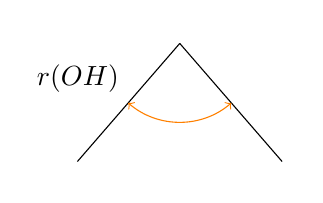
\begin{tikzpicture}
   \Odraw{0,1.5}
   \Hdraw{-1.3,0}
   \Hdraw{1.3,0}
%  \shade[inner color=blue,outer color=red] (0,0) rectangle (4,4);
%  \shadedraw[inner color=blue,outer color=red, draw=black] (0,0) rectangle (4,4);
  \draw(0,1.5) node[circle,minimum size=.4cm] (O) {};
  \draw(-1.3,0) node[circle,minimum size=.3cm,] (H1) {};
  \draw(1.3,0) node[circle,minimum size=.3cm,] (H2) {};
  %\draw(1.3,0) node[circle,minimum size=.2cm,draw,fill=blue] (H2) {};
  %\draw(.65,.8) node[circle,minimum size=.5cm,draw,fill=blue] (O) {};
 % \draw (A.center) -- (B.center);
\begin{pgfonlayer}{background}
 \draw (O.center) -- node[above left] {$\r(\te{OH})$}(H1.center);
 \draw (O.center) --  (H2.center);
  \draw pic["$\anghoh$", draw=orange, <->, angle eccentricity=1.2, angle radius=1.cm]
    {angle=H1--O--H2};
\end{pgfonlayer}
 \end{tikzpicture}
\end{equation*}
 \caption{The geometry of $\tip$ water. O is red, H is blue. Each atom coincides with a site with charge $q$ and
  LJ-paramteres $\eps$ and $\si$.}
\label{Fig:Theo:TIP3Geo}
\end{figure} 

When there is no bond formation or breaking to be expected, quantum mechanical
calculations can be replaced by classical calculation, that is the position
of the atomic cores is again a sharply determinable quantity and motion
is governed by forces. That is, all particles move in a classical potential.
We will only treat water molecules as classical particles, so we need a good
%% CHECK: Real source by Jorgensen? Or 1981 source?
classical model of water. We decided on the quite popular $\tip$ potential 
by Jorgensen \etal \cite{Jorgensen1983TIP3P}. The geometry can be
seen in Figure \ref{Fig:Theo:TIP3Geo}. The three sites of the $\tip$ potential
coincide with the atoms forming $\hto$. Each site has a charge $\qal$ with 
\ep{Coulomb interaction}
\begin{equation}
\EC(\ralbe)=\frac{1}{4\pi\eps_0}\frac{\qal\qbe}{\ralbe},
\label{Theo:TIP3EC}
\end{equation}
where $\al,\be$ are the site types and $\ralbe$ is the distance between
the sites $\al$ and $\be$. Sites also interact by Van-der-Waals forces
which are described by a \ep{Lennard-Jones} (LJ) potential
\newcommand\ELJ{\enmat V^{\te{LJ}}_{\al\be}}
\newcommand\salbe{\enmat{\si_{\al\be}}}
\newcommand\ealbe{\enmat{\eps_{\al\be}}}
\begin{equation}
\ELJ(r)=4\ealbe\ed{\rb{\frac{\salbe}{\ralbe}}^{12}-\rb{\frac{\salbe}{\ralbe}}^{6}}.
\label{Theo:TIP3ELJ}
\end{equation}
The original $\tip$ model only had LJ interaction between the oxygen atoms. In
the CHARMM \cite{CHARMM} implementation, the H atoms are LJ sites as well. Therefore,
a $\tip$ water molecule $i$ moves in the potential of all other $\tip$ waters by
%% CHECK: HERE WE ARE
\begin{equation}
V_i(\r_i)=\sum_{j\neq i} \sum_{\al,\be} \ed{\EC(\ralbe(\r_i,\r_j)) + \ELJ(\ralbe(\r_i,\r_j))}.
\label{Theo:TIP3Potential}
\end{equation}
The first sum runs over all other water molecules and the second over all sites in both
molecules. \eqref{Theo:TIP3Potential} only contains intermolecular interaction. There
would also be the possibility to include intramolecular degrees of freedom with
harmonic potentials for bond and angle stretching. This is not the case for $\tip$,
where all sites are fixed within the molecule, reducing the 9-dimensional coordinate
\mbox{$\r_i=\r_i\rb{\r_{\te O},\r_{\te H1},\r_{\te H2}}$} to a 6-dimensional one, \mbox{$\r_i=\r_i\rb{\r_{\te O},\Om}$}
with the orientational dependency described by $\Om\in\R^3$.

The parameters $\ealbe$, $\salbe$ and $\qal, \qbe$ as well as the geometric parameters
$\r(\te{OH})$ and $\anghoh$ define the $\tip$ potential. They are chosen to reproduce
(macroscopic) thermodynamic properties of a pure water system.
%% CHECK if heats. Wikipedia nennt eine andere Quelle dafür.
The CHARMM $\tip$
potential is fitted to yield good specific heats \cite{MacKerell1998CHARMMTIP3}.  

\subsection{QM/MM}
\label{Sec:Theo:QMMM}

We already motivated using both QM and MM calculations simultaneously due to
the speed of MM and the accuracy of QM results. The simultaneous use
demands some notion of coupling between the two systems. The original
QM/MM coupling scheme proposed by Warshel and Levitt \cite{Warshel1976QMMM}
is nowadays only one among several schemes.
%% CHECK: Dringend checken, ob das irgendwie stimmt.
We chose an approximation
in which the QM part was subject to the external potential defined
by the MM charges and the MM part interacted with the QM atoms by
the LJ potential \eqref{Theo:TIP3ELJ}. That way, the electrostatic
interaction is covered by the QM part while the MM part accounts for
VdW interaction.

\subsection{Energy Minima and Transition States}
\label{Sec:Theo:Minima}
Finding energy minima of the PES for QM or QM/MM systems is basically following
the path defined by the gradient (force)
\newcommand\RM{\enmat{\bo R^M}}
\begin{equation}
\bo F(\RM)=-\nabla V(\RM)
\label{Theo:ForceGradient}
\end{equation}
of the total system's energy $V(\RM)$, where $\RM$ is the vector containing
all atomic coordinates. Again, there is no knowing whether this leads to
a global or a local minimum.

When working on a computer, \eqref{Theo:ForceGradient} must be integrated
in a discretised form. This is best done with step sizes depending on the
value of $\bo F$ and of course one needs tolerances that define convergence.
We used the DL-FIND algorithm \cite{Kaestner2009} with the default tolerances
to follow the minimum energy path.

Evaluating the gradient in \eqref{Theo:ForceGradient} is fortunately not
expensive in comparison to a single energy evaluation of the QM part. The gradient of
the MM region can be calculated straighforwardly from \eqref{Theo:TIP3Potential}.
For the QM region, there are schemes to obtain analytical results for the gradient
for a given wave function \cite{Brorsen2014AnalyticalGradientDFT}.
%% CHECK: do they ignore QM/MM?

%% CHECK: Pre-reactive complex?
\newcommand\ebased[2]{exp(-(\x-#1)^2/#2)} 
\begin{figure}[tc]
%\includegraphics{
\tikzsetexternalprefix{TikzPics/Theo/}
\tikzsetnextfilename{Fig.Theo.PES} 
\begin{equation*}
\begin{tikzpicture}
  \draw[->] (-3.7,0) -- (5,0) node[right] {$\xi$};
  \draw[->] (-3.4,-.3) -- (-3.4,4.5) node[above] {$E$};
  \draw[domain=-2.4:4.1,smooth,variable=\x,blue] plot ({\x}, {1+3*\ebased{1}{1.5}-1*\ebased{2}{.6}+2*\ebased{4}{3}});%{4*\ebased{2}{3}});
  \draw[domain=4.1:4.3,smooth,variable=\x,blue] plot ({\x}, {3.0});%{4*\ebased{2}{3}});
  \draw[dotted] (2.3,-.1) node[below] {$\xi_{\te {MIN}}$} -- (2.3,4.3) ;
  \draw (1.9,1.87) -- (2.7,1.87) node[right] {$E_{\te {MIN}}$};
  \draw[dotted] (.9,-.1) node[below] {$\xi_{\te {TS}}$} -- (.9,4.3) ;
  \draw (.5,3.93) -- (1.3,3.93) node[right] {$E_{\te {TS}}$};
  \draw[dotted] (-2.4,-.1) node[below] {$\xi_{0}$} -- (-2.4,4.3) ;
  \draw (-2.6,1.004) node[left] {$E_{0}$} -- (-2,1.004) ;
\end{tikzpicture} 
\end{equation*}
 \caption{A cut of a PES along reaction coordinate $\xi$. The reaction coordinate starts
 at some initial $\xi_0$ with energy $E_0$ and follows a path of minimum energy.
 The minimum with $E_{\te{MIN}}$ is located at $\xi_{\te{MIN}}$. The transition state with $E_{\te{TS}}$
 is a maximum at $\xi_{\te {TS}}$.}
\label{Fig:Theo:PES}
\end{figure} 

To evaluate our model, we will also calculate a \ep{transition state} (TS). This
is the state of maximum energy along a \ep{reaction path}, that is a path that
starts at some initial geometry with initial \ep{reaction coordinate} $\xi_0$
and then follows the negative gradient to a maximum (the transition state) and
after that reaches a new minimum by continuing on its route along the
gradient. In Figure \ref{Fig:Theo:PES}, an example of such a path between
reaction coordinates $\xi_0$ and $\xi_{\te{MIN}}$ is plotted. 

%% CHECK: ZITAT. Außerdem Theorie checken!
In this work, we obtain transition state with the \ep{dimer method} \cite{DimerMethod}. It uses two
images of the system with a slight offset, then rotates them to find the minimum 
eigenvalue of the Hessian matrix \eqref{Theo:Hessian}. It follows these ``gradients" 
by an iterative scheme a saddle point is reached. This is the transition state.

Transition states are important for calculating tunneling rates. These are interesting
for the analysis of molecule formation on ice surfaces since at temperatures as low
as in the interstellar medium, tunneling has a significant contribution to the dynamics of 
these systems.

\subsection{Technical Details}

%% CHECK: Sollte nwchem noch rein?
Before proceeding to actual calculations, we want to mention the programs and tools 
used for these. As we already mentioned, the optimizations are carried out with
DL-FIND \cite{Kaestner2009}, as are the dimer method and the calculation of 
Hessian matrices. DFT calculations are performed with TURBOMOLE\cite{TURBOMOLE}.
Force field calculations are performed by CHARMM \cite{CHARMM2009}. These programs were interfaced
via ChemShell \cite{chemshell}, which also provided the QM/MM coupling.

For the post-HF calculations in the benchmark, we used the MOLPRO \cite{MOLPRO_brief}
package.

All molecular visualizations are created with VMD \cite{HUMP96}.


%\subsection{The Fletcher Surface}
%\label{Sec:Theo:Fletcher}

\section{Benchmarking}
\newcommand\htohto{\enmat{\hto-\hto}}
\newcommand\htoh{\enmat{\hto-\te H}}
\label{Sec:Bench}

In the previous section, we did introduce the basic notions of the theoretical structure underlying our
computations. We did already mention that DFT functionals and basis sets are of great importance
to the accuracy of our calculations. Unfortunately, not much can be said a priori about
which functional combined with which basis set should be used to describe a certain system.
There are recommendations as some functionals were fitted to best represent a certain
group of elements or reactions, but in order to determine the reliability of the
later results, there is no way around literature research and own benchmark tests.

We already
discussed the functionals we want to test in Section \ref{Sec:Theo:Functionals}, and we
have reason to hope that at least the \pbez, $\pw\dt$ and $\bns\dt$ functionals will be sufficiently
accurate to describe water-water interaction, as they are recommended by Anacker and Friedrichs \cite{Anacker2014}.
We did also already name the basis sets we want to compare alongside the functionals in Section \ref{Sec:Theo:Basis}.

We used two different benchmarks, namely the interactions energies of an $\htohto$ and an $\htoh$ system.
The reference calculations were in both cases performed MOLPRO \cite{MOLPRO_brief} calculations
at the $\ccsdtf$ \cite{CCSDTF12} level of theory with the $\vtz$\cite{VTZ} basis set, for
which we found energy minima. 
%We used these minima as initial geometries for two different
%types of reference calculations:
%% CHECK: Sollte man Benchmark i. überhaupt erwähnen? Meine Schlussfolgerung: Nein.
%\begin{enumerate}[i.]
%  \item Energy reference: No minimization was performed. Instead, the $\ccsdtf/\vtz$ geometries
%    were used and the energy values are compared.
%  \item Geometry reference: The initial geometries were further optimized to arrive at a minimum
%    geometry and energy corresponding to the DFT method.
%\end{enumerate}

We performed the same calculations at the DFT level of theory with different basis sets. The results can be compared
to the coupled-cluster data with respect geometry and energy deviations. We will discuss these for the cases $\htohto$ and $\htoh$
separately.

%% CHECK: Source?
Note that, obviously, the coupled cluster results are approximations just as the DFT results, however
there is good reason to assume that they are more accurate. For the following comparisons, we will
therefore consider the coupled cluster results as if they were the correct values for this
interaction.

\subsection{$\htoh$ Interaction}

\tikzsetexternalprefix{TikzPics/Benchmark/}
\tikzsetnextfilename{Fig.Bench.H2O+H.NoD3}
\pgfplotsset{xtick style={draw=none}}

\begin{figure}[h]
\centering
\begin{tikzpicture}
\begin{axis}[
    height=8cm,
    width=.5*\textwidth,
    ybar,
    xmin=.5,
    xmax=10.5,
    ybar=0pt,
    axis x line*=bottom,
    enlarge x limits=0.015,
    enlarge y limits=0.15,
    legend pos=south west,
    legend style={legend columns=2},
    ylabel={interaction energy deviation $\Delta \eint$ / kJ/mol},
    xticklabels={\btlyp,\bns,\bhlyp,\blyp,\bp,\pbe,\pbez,\tpss,\tpssh,\pw},
    xtick=data,
    grid=minor,
    xticklabel style={rotate=90},
    bar width = .008*\textwidth,
    minor xtick={1.5,...,9.5},
    yticklabel pos=left,
    grid style={dotted,gray},
    ymajorgrids=true,
    ]
\addplot[green!20!black,fill=green!80!white] coordinates {(1,-1.3372721700) (2,.4102606300) (3,-.7425176550) (4,-1.8385326300) (5,-2.6576361200) (6,-1.8459102850) (7,-.8015651500) (8,-7.2262161600) (9,-5.3374052050) (10,-.2959201050) };
\addplot[blue!20!black,fill=blue!80!white] coordinates {(1,-.4004150050) (2,.4550516600) (3,-.0939141350) (4,-.8160841650) (5,-3.0162006550) (6,-.5095570400) (7,-.0395662850) (8,-8.7172901200) (9,-6.5151519950) (10,-.1592628300) };
\addplot[red!20!black,fill=red!80!white] coordinates {(1,.1896136100) (2,.4029354850) (3,.2102500400) (4,.3640780850) (5,-2.1326673950) (6,-.8015388950) (7,-.1888522150) (8,-7.3249349600) (9,-5.3460956100) (10,.0254673500) };
\addplot[yellow!20!black,fill=yellow!80!white] coordinates {(1,-.1378124950) (2,.4396399750) (3,.0877967200) (4,-.2670658600) (5,-2.6442460700) (6,-.6816060550) (7,.0698645550) (8,-8.0693954850) (9,-5.9672889100) (10,-.0466813900) };
\legend{def2-SVPD,def2-TZVP,def2-TZVPD,def2-QZVP}
\end{axis}
\end{tikzpicture}
%\captionsetup{format=hang}
%\setcapmargin[4cm]{1cm}
\caption{The $\htoh$ benchmark results for different basis sets without dispersion correction.
Energies are plotted as differences to the reference energy from $\ccsdtf/\vtz$ calculations,
see \eqref{Bench:RefEnergy}.}
\label{Fig:Bench:H2O+H:NoD3}
\end{figure}

First information about $\htoh$ interaction can be found in Figure \ref{Fig:Bench:H2O+H:NoD3}, where
we compared functionals (without dispersion correction) in different basis sets. We compared
energy values of the form
\newcommand\ecc{\enmat{\eint_{\te {CC}}}}
\begin{equation}
\Dl\eint=\eint\dft-\ecc.
\label{Bench:RefEnergy}
\end{equation}
$\eint\dft$ stands for the interaction energy of the system computed with a certain
DFT functional and basis set, and $\ecc$ is the interaction energy with $\ccsdtf/\vtz$.
For $\htoh$, we found $\ecc=-0.455 \te{ kJ/mol}$, so we have an only
weakly bonded system. Figure \ref{Fig:Bench:H2O+H:NoD3} does not contain our results
for the def2-SVP basis set since they are much worse than all other results --
up to 20 $\kmo$ and usually more than 5 $\kmo$. Only the $\bhlyp$, $\pbez$ and
$\pw$ functional had errors between 2 and 5 $\kmo$. However,
the additional of diffuse functions effects quite a remarkable improvement to the
def2-SVP results, such that def2-SVPD calculations are well comparable to higher
results obtained with bigger basis sets. Another more general result is that the inclusion
of the D3 dispersion correction is not beneficial to the interaction
energy values of $\htoh$, which can be seen by comparing Figure \ref{Fig:Bench:H2O+H:NoD3}
to Figure \ref{Fig:Bench:H2O+H:D3}. The contribution of dispersion in $\htoh$
is therefore overestimated by the dispersion correction.

Concerning basis sets, it is also
noteworthy that def2-QZVP does not seem to offer a clear advantage over the
other three basis sets in both figures. With additional dispersion,
it tends to yield similar accuracy as def2-TZVP, while being inferior
to def2-TZVPD for most functionals. Still, without dispersion correction,
it is as good as def2-TZVPD or slightly better, while it takes approximately
1.5 times as long to complete a single SCF iteration. From a first glance
at the ``better'' functionals in this case, one could therefore consider
the def2-TZVP and def2-TZVPD basis sets as good compromises between
accuracy and computational cost among the selection presented. 

\tikzsetexternalprefix{TikzPics/Benchmark/}
\tikzsetnextfilename{Fig.Bench.H2O+H.D3}
\begin{figure}[h]
\centering
\begin{tikzpicture}
\begin{axis}[
    height=8cm,
    width=.5*\textwidth,
    ybar,
    xmin=.5,
    xmax=10.5,
    ybar=0pt,
    axis x line*=bottom,
    enlarge x limits=0.015,
    enlarge y limits=0.15,
    legend pos=south west,
    legend style={legend columns=2},
    ylabel={interaction energy deviation $\Delta \eint$ / kJ/mol},
    xticklabels={\btlyp-D3,\bns-D3,\bhlyp-D3,\blyp-D3,\bp-D3,\pbe-D3,\pbez-D3,\tpss-D3,\tpssh-D3,\pw-D3},
    xtick=data,
    grid=minor,
    xticklabel style={rotate=90},
    bar width = .008*\textwidth,
    minor xtick={1.5,...,9.5},
    yticklabel pos=left,
    grid style={dotted,gray},
    ymajorgrids=true,
    ]
\addplot[green!20!black,fill=green!80!white] coordinates {(1,-1.9265919000) (2,.3747901250) (3,-1.1717343950) (4,-3.5689471700) (5,-3.8726650100) (6,-2.6704748150) (7,-1.6286239050) (8,-9.0398327950) (9,-7.2252184700) (10,-.6478683800) };
\addplot[blue!20!black,fill=blue!80!white] coordinates {(1,-2.7286033850) (2,.3730572950) (3,-1.3828771050) (4,-4.3534203150) (5,-6.0301696350) (6,-1.4111799950) (7,-.8765494300) (8,-10.4059067000) (9,-8.2939545000) (10,-.5181686800) };
\addplot[red!20!black,fill=red!80!white] coordinates {(1,-1.4858754700) (2,.3724796850) (3,-1.0818897850) (4,-3.1681383400) (5,-5.2421520650) (6,-1.6039442050) (7,-.9737191850) (8,-9.0033120900) (9,-7.1565879000) (10,-.2545159700) };
\addplot[yellow!20!black,fill=yellow!80!white] coordinates {(1,-2.4036189950) (2,.4046945700) (3,-1.2088327100) (4,-3.7478224850) (5,-5.6954708950) (6,-1.3377972700) (7,-.9505097650) (8,-9.7233292100) (9,-7.7258225550) (10,-.3410524500) };
\legend{def2-SVPD,def2-TZVP,def2-TZVPD,def2-QZVP}
\end{axis}
\end{tikzpicture}
\caption{The $\htoh$ benchmark results for different basis sets including dispersion correction.
Energies are plotted as differences to the reference energy from $\ccsdtf/\vtz$ calculations,
see \eqref{Bench:RefEnergy}.}
\label{Fig:Bench:H2O+H:D3}
\end{figure}

Let us now look at the different functionals.  The $\bns$ and
$\pw$ functionals yield good approximations to $\ecc$ with and without
dispersion corrections. The results do not vary strongly with basis set size,
however they are slightly more accurate for the def2-TZVPD basis set, which
is computationally much faster than the def2-QZVP basis set (which takes roughly
1.5 times the computation time of the smaller basis set). The $\bhlyp$ functional
yields good results as well, although $\bhlyp\dt$ is significantly less accurate.
The $\pbez$ functional behaves similarly, and describes the system very accurate only
without the dispersion correction.
The $\tpss$ and $\tpssh$ functionals should not be used to describe this interaction,
while $\btlyp$ and $\blyp$ can be considered quite good -- not as good as $\bns$,
$\pw$ or $\pbez$ but much better than $\tpss$ and $\tpssh$ -- while they become
worse with additional dispersion.

So from the $\htoh$ data, one can already conclude that the $\tpss$ and $\tpssh$
functionals should not be expected to yield good energy values for hydrogen adsorption,
which may however still occur due to error cancellation. Furthermore, the def2-SVP basis
set is not fit to describe $\htoh$ interaction. Since they are sufficiently accurate
while not too expensive, we will especially evaluate the def2-TZVP basis set family
for $\htohto$ interaction.
%% CHECK: Table mit Computation times?
%% CHECK: RMSD table?

\subsection{$\htohto$ Interaction}

\tikzsetexternalprefix{TikzPics/Benchmark/}
\tikzsetnextfilename{Fig.Bench.H2O+H2O.TZVPCompare}
\begin{figure}[h]
\centering
\begin{tikzpicture}
\begin{axis}[
    height=8cm,
    width=.5*\textwidth,
    ybar,
    xmin=.5,
    xmax=10.5,
    ybar=0pt,
    axis x line*=bottom,
    enlarge x limits=0.015,
    enlarge y limits=0.15,
    legend pos=north east,
    legend style={legend columns=2},
    ylabel={interaction energy deviation $\Delta \eint$ / kJ/mol},
    xticklabels={\btlyp,\bns,\bhlyp,\blyp,\bp,\pbe,\pbez,\tpss,\tpssh,\pw},
    xtick=data,
    grid=minor,
    xticklabel style={rotate=90},
    bar width = .008*\textwidth,
    minor xtick={1.5,...,9.5},
    yticklabel pos=left,
    grid style={dotted,gray},
    ymajorgrids=true,
    ]
\addplot[blue!20!black,fill=blue!80!white] coordinates {(1,-2.2911688300) (2,1.8945608000) (3,-3.3056620300) (4,-1.3177384500) (5,-1.2830293400) (6,-4.9496451100) (7,-3.7824003200) (8,-2.2352456800) (9,-2.0561340700) (10,-2.4866635600) };
\addplot[blue!20!black,pattern color=blue!80!white,pattern = horizontal lines] coordinates {(1,-5.3662069400) (2,-3.1298060400) (3,-5.7434387800) (4,-5.0291977600) (5,-4.7869166200) (6,-6.8055060400) (7,-5.7431237200) (8,-4.8009367900) (9,-4.5759839500) (10,-3.8439420400) };
\addplot[red!20!black,fill=red!80!white] coordinates {(1,1.6138948500) (2,5.9163017000) (3,.0413778800) (4,3.1551158600) (5,2.9033304100) (6,-.6073831700) (7,-.1202479000) (8,1.6705531400) (9,1.6996436800) (10,1.2347726500) };
\addplot[red!20!black,pattern color=red!80!white,pattern = horizontal lines] coordinates {(1,-1.4527941700) (2,.9033820400) (3,-2.3888899400) (4,-.5200065300) (5,-.7710043300) (6,-2.4600935000) (7,-2.0844369600) (8,-.8217289900) (9,-.8236718600) (10,-.1117937900) };
\legend{def2-TZVP,def2-TZVP+D3,def2-TZVPD,def2-TZVPD+D3}
\end{axis}
\end{tikzpicture}
\caption{The $\htohto$ benchmark results for the def2-TZVP and def2-TZVPD basis sets.
The dashed results include dispersion corrections. Energies are plotted as differences
to the reference energy from $\ccsdtf/\vtz$ calculations, see \eqref{Bench:RefEnergy}.}
\label{Fig:Bench:H2O+H2O:TZVPCompare}
\end{figure}

Again, we compare energies to the reference energy as in \eqref{Bench:RefEnergy}. The
reference energy for the $\htohto$ dimer is at \mbox{$\ecc=-20.982\ \kmo$}.
In Figure \ref{Fig:Bench:H2O+H2O:TZVPCompare}, we take a look at the differences between
dispersion corrected and not dispersion corrected results in the def2-TZVP and def2-TZVPD
basis sets. It becomes immediately apparent that the results here differ stronger from
the reference energy than in the $\htoh$ case. For the functionals without dispersion
correction, this may well be due to the more important role of dispersion for this interaction. 
But inclusion of the dispersion correction does not resolve the issue for most cases,
it often happens that dispersion yields bonds that are much too attractive. This
is most striking for the def2-TZVP basis set, which generally predicts too attractive
interaction for all functionals but $\bns$.

 
\newpage

\section{Adsorption on the Ice Surface}
\label{Sec:Ads}

\subsection{The Surface Model}
\label{Sec:Ads:Model}

\subsection{Results}
\label{Sec:Ads:Results}

\section{Conclusion}
\label{Sec:Con}

\section*{Acknowledgment}
I want to thank Professor J. Kaestner for his support and Mr. Jan Meisner for
his introduction to the topic and his company along the way.


%\clearpage
% \bibliographystyle{apalikenotitle}
\bibliographystyle{ieeetr}
% \begin{thebibliography}
\bibliography{MasterBib}

\end{document}

%\begin{figure*}[t]
%\centering
%\begin{tikzpicture}
%\begin{axis}[
%height=8cm,
%width=15cm,
%    ybar,
%    xmin=.5,
%    xmax=10.5,
%%    axis y line*=left,
%    axis x line*=bottom,
%    enlarge y limits=0.15,
%    legend style={at={(0.5,-0.15)},
%      anchor=north,legend columns=-1},
%    ylabel={interaction energy deviation $\Delta \eint$ / kJ/mol},
%    xticklabels={b3lyp,b97-d,bhlyp,blyp,bp86,pbe0,pbe96,tpss,tpssh,pw6b95},
%    xtick=data,
%%    extra x ticks={1.5,...,9.5},
%  %  extra x ticks labels={\empty},
%    grid=minor,
%    %xticklabel interval boundaries,
%    %x tick label style={rotate=45,achor=east}
%    %nodes near coords,
%    %every node near coord/.append style={rotate=90, anchor=west},
%    bar width = 6pt,
%    minor xtick={1.5,...,9.5},
%    yticklabel pos=left,
%grid style={dotted,gray},
%    ymajorgrids=true,
%%    minor x tick num=1,
%    ]
%\addplot[brown!20!black,fill=brown!80!white] coordinates {(1,-5.9330523900) (2,7.2492943050) (3,-3.1331666800) (4,-9.8480667150) (5,-11.0948116450) (6,-2.1139475800) (7,-5.1825532150) (8,-18.4540356350) (9,-15.1383704500) (10,-2.7420196900) };
%\addplot[yellow!20!black,fill=yellow!80!white] coordinates {(1,-1.3372721700) (2,.4102606300) (3,-.7425176550) (4,-1.8385326300) (5,-2.6576361200) (6,-.8015651500) (7,-1.8459102850) (8,-7.2262161600) (9,-5.3374052050) (10,-.2959201050) };
%\addplot[green!20!black,fill=green!80!white] coordinates {(1,-.4004150050) (2,.4550516600) (3,-.0939141350) (4,-.8160841650) (5,-3.0162006550) (6,-.0395662850) (7,-.5095570400) (8,-8.7172901200) (9,-6.5151519950) (10,-.1592628300) };
%\addplot[blue!20!black,fill=blue!80!white] coordinates {(1,.1896136100) (2,.4029354850) (3,.2102500400) (4,.3640780850) (5,-2.1326673950) (6,-.1888522150) (7,-.8015388950) (8,-7.3249349600) (9,-5.3460956100) (10,.0254673500) };
%\legend{def2-SVP,def2-SVPD,def2-TZVP,def2-TZVPD}
%\end{axis}
%\end{tikzpicture}
%\end{figure*}